\subsection*{Generaliszed complex sinusoid}
class notes: jan 19, 2016

$s(t) = e^{-t/\tau}e^{j\omega_0 t}$

%S plane: $s_0 = \sigma_0 + j\omega_0$ and $\simga = -\frac{1}{\tau_0}$

Sample it: $ \leftarrow$

$s(nt) = \alpha * e ^{-nT/\tau_0}e^{j\omega_0 n T}$
$s(nt) = \alpha * (e ^{T/\tau_0})^n(e^{j\omega_0T})^n$


Define: $Z_0 = r_0 e^{j\omega_0}$

i.e, $Ae^{s_0 n T} = AZ_0^n$ s-0dervived and z-derived, respectively.

$Z_0 = e^{S_0 T}$  

\mbox{$s \leftrightarrow z$ map}

$a e^{s_0 t} \rightarrow SAMPLE_t \rightarrow Ae^{s_0 n T}$

$\stackrel{\Delta}{=} A Z_0^m$

$e^T{\sigma_0 + j[\omega_0 + k2\pi fs ]}$\\
$e^T{\sigma_0 T} * e^{j\omega_0}e^{jk}$ \paulhint{not done yet}

This thing aliases, and he jsut wrote a proof why. \paulhint{But... why?}

Add the "strips" together to get the digital domain.



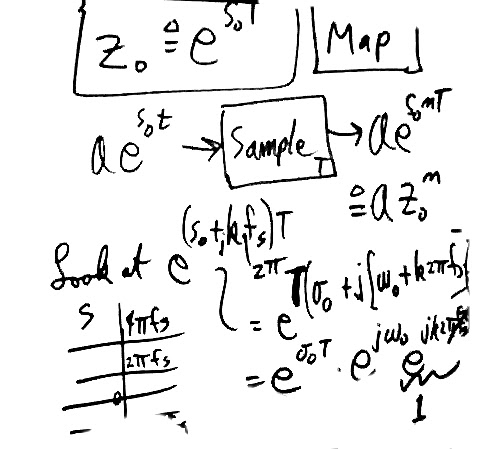
\includegraphics[scale=0.5]{photos/jan17/9a}



$S \leftrightarrow Z$ How?

$z_0 = e^{s_0 T}$ \\

clue: Diff. thm for laplace xf.

\paulhint{how do we prove that a thing doesn't alias?}

$S = \frac{1 - z^{-1}}{T}$

This is called a "Backward Euler", which has the advantage of being causal. The foward Euler (look ahead) needs a + instead of a minus. There's also a Center Euler.

Centered Euler: $\frac{x_{n + 1} - x_{n - 1}}{2T}$

\subsection*{Derivative}

\paulhint{See pictures taken at aroudn 15:35 PST... 9a}


\josquote{For a derivative to exist, it must be unique}

B and F stands for backward and foward.


Four mapping:

sample mapping.

backward euler.

forward euler.

centered approximation. (this onen goes up in order).

\subsection*{Trapezoidal}

step function with samples.  

simple thing is summing the areas x1, x2, x3.

Zero-order integral is to sum the rectangular areas.

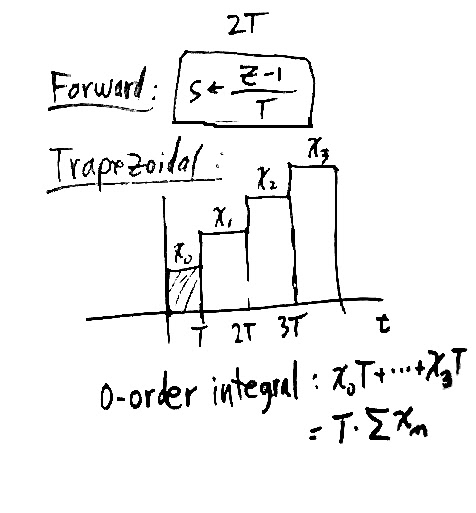
\includegraphics[scale=0.5]{photos/jan17/9b}

First order integral: We want to do a linear interpolation.
Corner to corner. 

We need the areas of the triangles. 

Here is how we do it:

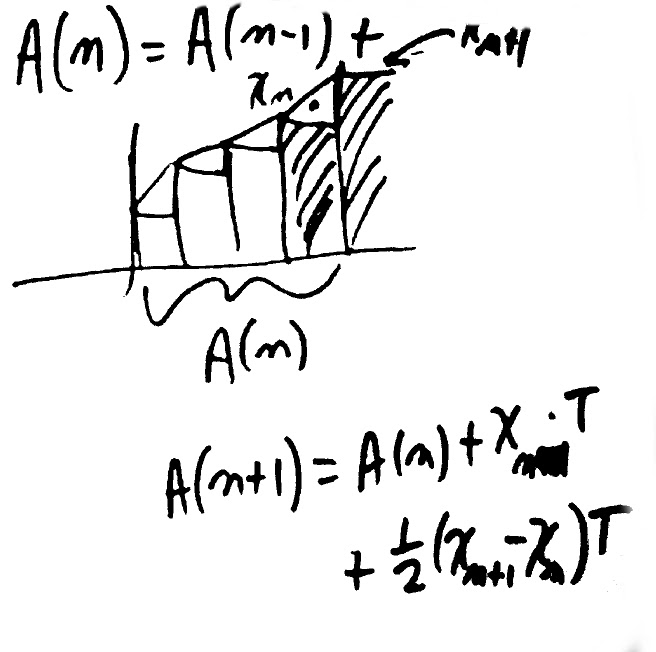
\includegraphics[scale=0.25]{photos/jan17/9i}

This can now be simplified:

$=A(n) + \frac{1}{2}X_{n + 1}T + \frac{1}{2}x_nT$

Trying to see if this turns into the recursion that JOS likes:
$y(n) = y(n -1) + \frac{T}{2}[x_{n + 1} + x_n]$

%Simplifies to form \paulhint{see picture taken at about 3:50. woops didn't catch it.}


Let's take the Z transform using the shift thereom:

$(\frac{1 - Z^ -1}{T})Y(z) = (\frac{1 + z^{-1}}{Z})X(x)$ \\

$H(z) \stackrel{\Delta}{=} \frac{Y(z)}{X(x} = 
\frac{2}{T} \frac{1 - z^{-1}}{1 + z^{-1}}$
Firt order numerical intergration

The first thing you try to do with he S plane (analogue) to the Z plane (digital, discrete) is the bilinear transform. 

Two point average on your signal. 

It's a non-aliasing transformation from the S plane to the Z plane. 


\subsection*{Differentiation}

$x(t) \rightarrow \frac{d}{dt} \rightarrow x(dot)(t) $ \\

$x(t) \leftrightarrow X(s)$
$x(t)(dot) \leftrightarrow sX(s) - x(0) \rightarrow sX(s) $

\paulhint{picture taken at 15:57. Not sure where I am in the lecture 9c }

This is predictive:


$H(z) = \frac{1 - Z^{-1}}{T}$ \\
$H(e^{j \omega T}) = \frac{1 - e^{-j \omega T}}{T}$

\paulhint{see two pictures taken at 16:01 for rest of derivation 9d and 9e}

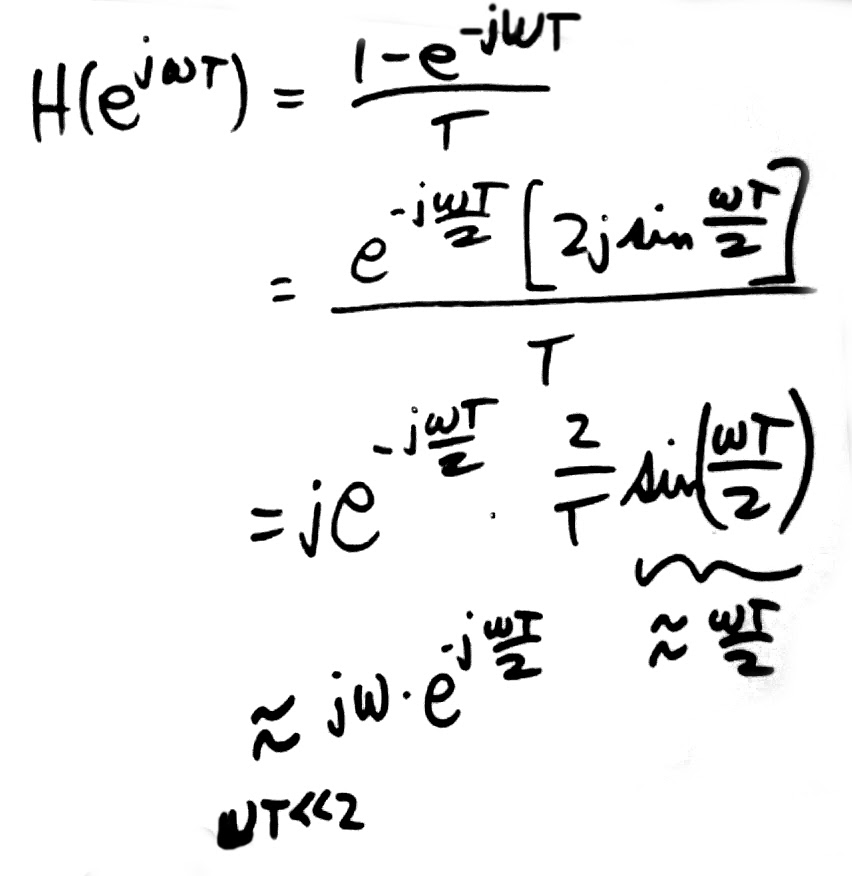
\includegraphics[scale=0.25]{photos/jan17/9d}

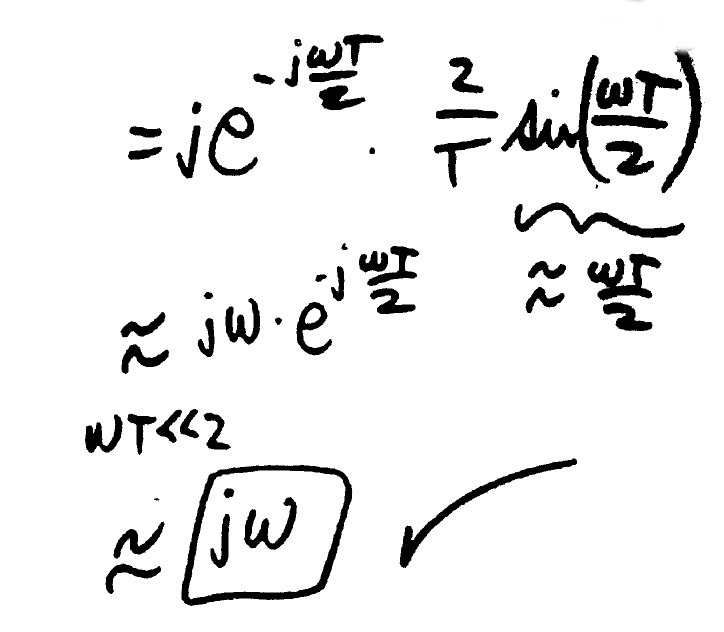
\includegraphics[scale=0.25]{photos/jan17/9e}

\paulhint{look up frequency warping... possibly covered after break}

\josquote{Time was invented to keep everything at once.}

\josquote{Cosmic moments. (Excuse for not doing homework:) It is Written.}

\subsection*{Frequency Warping}

Reminder of what we've seen:

We've seen derivitive of a filter \paulhint{?? this might not be right}

We can approximate the first-order differential equation in many ways. This
is whewre we get the forward/backward euler. 

First order is really nice because it is a noce 1:1 mapping of the S to the Z plane. No aliasing. 

Non-aliasing quarter preserving approximations. 

The really good one is the bilinear transform. 

The ideal differentiator is the + 6db/octave order filter. 

\paulhint{Bilinear transform, backwards euler, etc, are all from the moebius transform, so look up the moebius transform. There's apparently a mindblowing
video on the moebius transform.}

\paulhint{Bilinear transform with anotations (2pt avrage and drvt) see picture taken at 14:32}

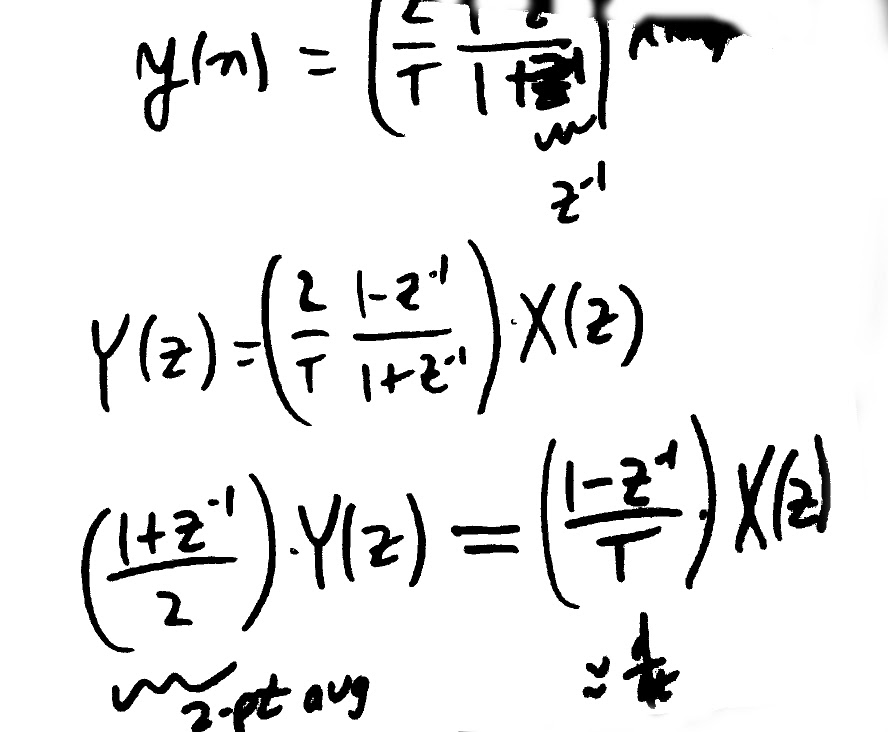
\includegraphics[scale=0.25]{photos/jan17/9j}

\josquote{Bilinear transform is known as the sandwich because it is a BLT (lol)}

\paulhint{Look up trapezoidal rule of derivation.}


graphing s-plane and z plane.

dc is perfectly mapped:

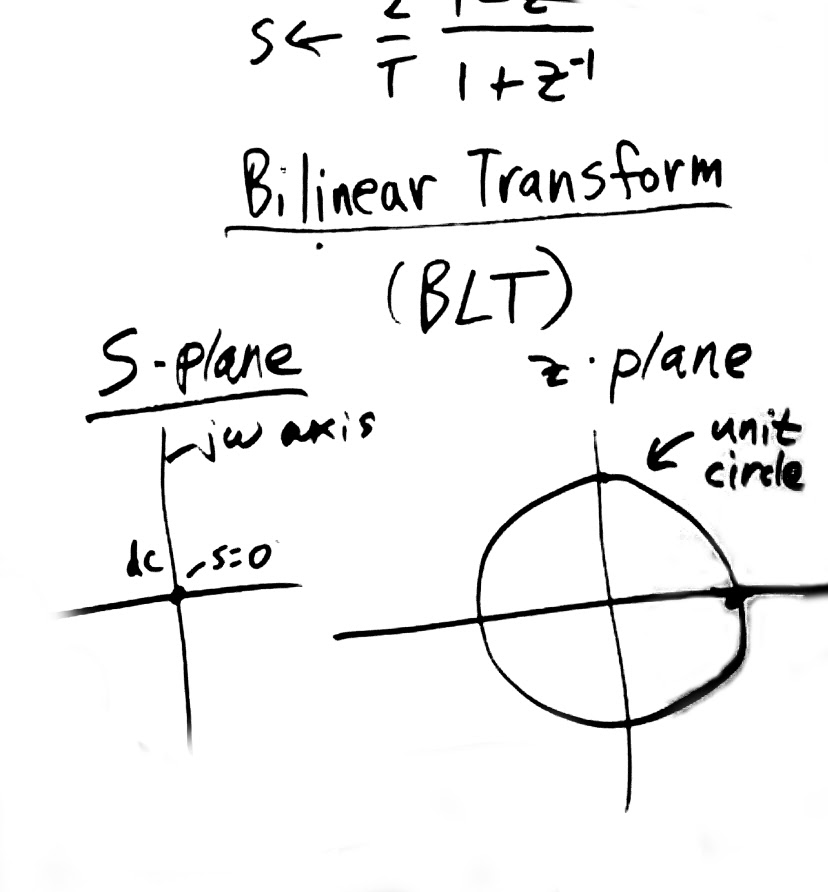
\includegraphics[scale=0.25]{photos/jan17/9f}

half the sampling rate: 

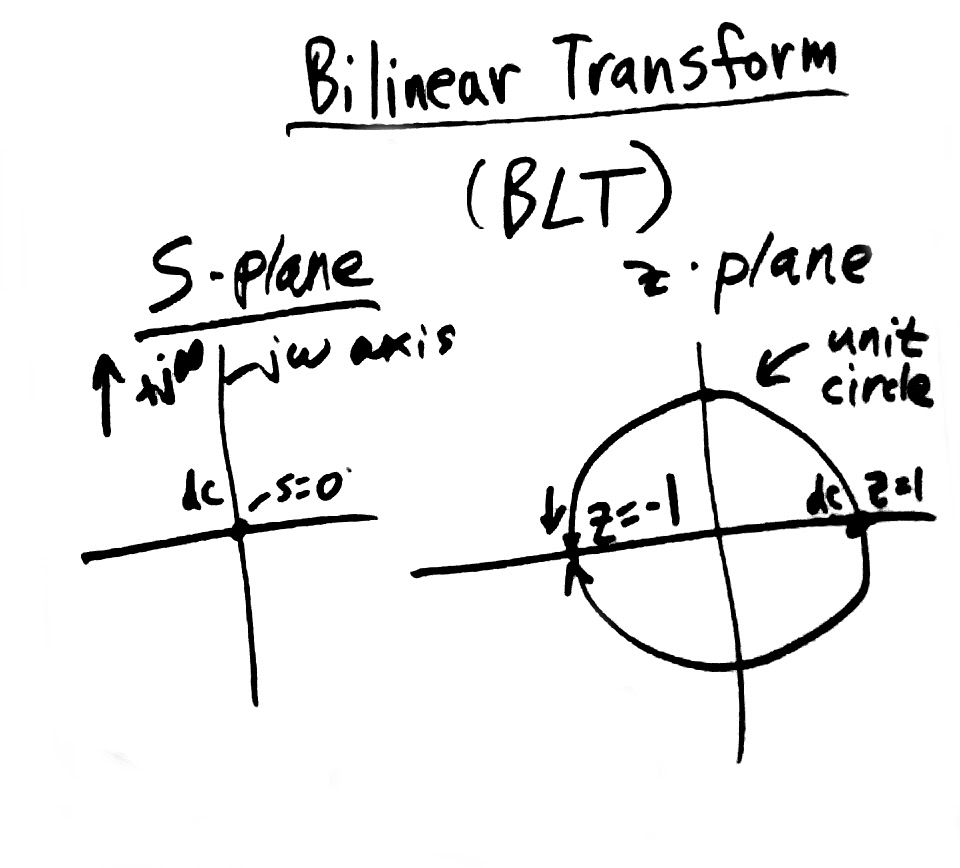
\includegraphics[scale=0.25]{photos/jan17/9g}

BLT: $\frac{s}{a} = \frac{1 - z^{-1}}{1 + z^{-1}}
= \frac{j\omega_a}{a} \stackrel{?}{=}
\frac{1 - e^{-j \omega_a T}}{1 + e^{-j \omega_a T}}$

\josquote{Alpha is just doint frequency scaling, that's all it can do.}
Known true for $w_a = 0, a, \inf$

See picture taken at 16:43 for rest of simplification.

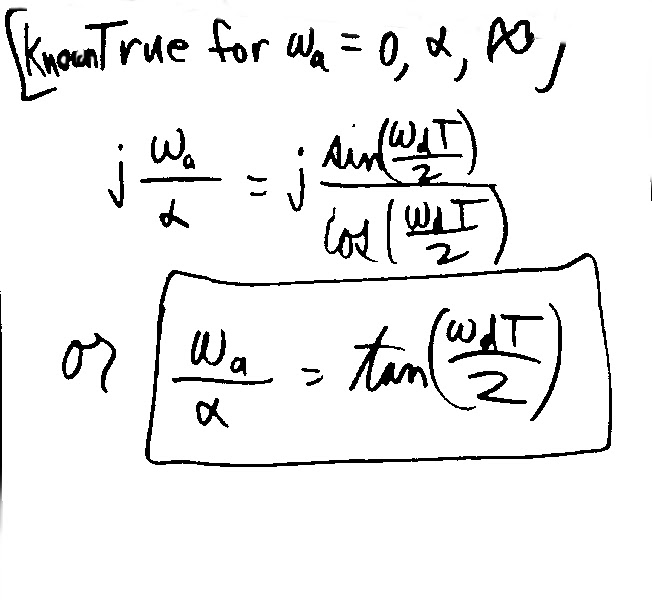
\includegraphics[scale=0.25]{photos/jan17/9h}

\paulhint{This was apparently a homework problem?}


If you change alpha, you change where low frequencies are. 

Alpha is one degree remaining of freedom for tuning a frequency. 

\paulhint{look up the mappings}
